\subsection{PSNR, SSIM and LPIPS metrics}

\begin{table*}[ht]
	\begin{center}
		\begin{tabular}{c|ccccccc}
			& \textbf{Baseline w/c}&\textbf{Baseline} & \textbf{Dahl} & \textbf{Eccv16} & \textbf{Siggraph17} & \textbf{ChromaGAN} & \textbf{InstColorization}  \\
			\midrule
			\textbf{PSNR} & - & - & 16.87 & 20.88 & 22.19 & 21.66 & 21.41 \\
			\midrule
			\textbf{SSIM} & - & - & 0.56 & 0.86 & 0.87 & 0.87 & 0.88 \\
			\midrule
			\textbf{LPIPS} & 0.28 & 0.28 & 0.36 & 0.23 & 0.20 & 0.21 & 0.23 \\
		\end{tabular}
	\end{center}
	\caption{{\small  Summary of the PSNR, SSIM and LPIPS metrics computed on the different models.}}
	\label{tab:metrics}
\end{table*}

We computed the following metrics:
\begin{itemize}
	\item Peak Signal-to-Noise Ratio (PSNR) \cite{psnr-ssim} computes the ratio between the maximum possible power of a signal and the power of corrupting noise that affects the fidelity of its representation. This is insufficent for assessing structured outputs such as images, as it assumes pixel-wise independence.
	
	\item Structural Similarity (SSIM) \cite{psnr-ssim} is based on human-like perceived changes in structural information, based on the fact that the pixels have strong inter-dependencies that carry important information about the structure of the objects in the visual scene. However, human judgments of similarity are context-dependent and may not actually constitute a distance metric \cite{met}.

	\item Learned Perceptual Image Patch Similarity (LPIPS) \cite{lpips} evaluates the distance between image patches, so that small values indicates that the colorized images are similar to the corresponding original images. This innovative approach exploits the internal activations of networks trained for high-level classification tasks (as AlexNet), corresponding to human perceptual judgments. Figure \ref{fig:lp} shows the computations needed.

\end{itemize}

\begin{figure}[h]
	\centering
	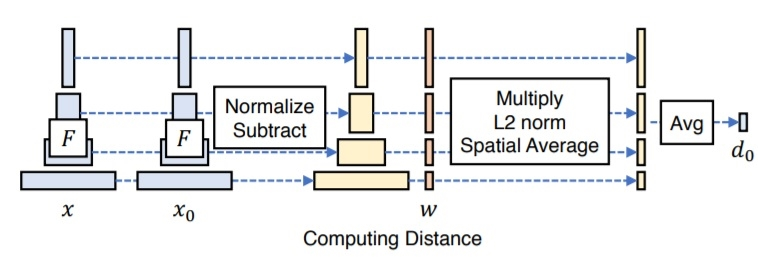
\includegraphics[width=8cm]{lpips.jpg}
	\caption{To evaluate the distance $d_0$ between two images, $x$ and $x_0$, given a network
		$\mathcal{F}$, LPIPS first computes deep embeddings, then normalizes the activations in the channel dimension, scales each channel by a vector $w$, and takes the $\ell_2$ distance. Then it performs the average across spatial dimension and across all layers.}
	\label{fig:lp}
\end{figure}

In order to get general results, the metrics were computed on the ri-colorized images from a heterogeneous dataset containing all the data available. Since PSNR and SSIM require a heavy computation, we decided to evaluate the baseline only with LPIPS, which is indeed the most significant metric.

As we can see from Table \ref{tab:metrics}, the best models according to LPIPS are Siggraph17 and ChromaGAN, which are indeed the highest-scored model in the Turing Test with human partecipants (see next section). This evaluation is also confirmed by PSNR. On the other hand, SSIM indicates InstColorization as best-performing model, followed by ChromaGAN and Siggraph17.

Dahl's model is the worst-performing for all the metrics, due to its desaturated results.
Notably, the baseline is able to outperform it and in general there's a grat gap between its scores and the other models' scores. However, this is most probably due to the reshaping of its colorized images ($224\times224\times3$) to match the original images ($256\times256\times3$) causing a little corruption of the results.
